% !TEX root = main.tex

Buildings are at the heart of society and currently account for 32\% of global final energy consumption and 19\% of energy related greenhouse gas emissions \cite{IPCC}. Nevertheless the building sector has a 50-90\% emission reduction potential using existing technologies, and widespread implementation could see energy use in buildings stabilise or even fall by 2050 \cite{IPCC}. Within this strategy, building integrated photovoltaics (BIPV) has the potential of providing a substantial segment of a building's energy needs \cite{defaix2012technical}. Even the photovoltaic (PV) industry has identified BIPV as one of the four key factors for the future success of PV \cite{raugei2009life}. \\

Recent developments regarding efficiency and costs of thin film BIPV technologies, in particular, CIGS, have brought new design possibilities \cite{NREL} \cite{kushiya2014cis} \cite{kaelin2004low} \cite{jelle2012building}. Their lightweight nature and customisable shapes allow for easier and more aesthetically pleasing integration into the building envelope. In addition, less power is required to actuate them, thus facilitating the development of dynamic envelope elements due to their reduced weight \cite{rossi2012adaptive}. \\


% \textcolor{cyan}{The PV industry is currently dominated by crystaline silicon photovoltaic cells due to their high efficiency and low processing costs \cite{saga2010advances}. However these technologies are often difficult to integrate in a way that maintains the architectural expression of the building \cite{Lueling2009ee}. This combined with their intrinsic weight restricts their large scale implementation to roofs where they are out of sight. However,} in the last decade, there has been interesting developments in second generation thin film technologies \cite{NREL}. In particular, Cu(In,Ga)Se$_2$ (CIGS) is reaching  competitive levels of efficiencies \cite{kushiya2014cis} and manufacturing costs \cite{kaelin2004low} \cite{jelle2012building}.\\



Dynamic buildings envelopes have gained interest in recent years because they can save energy by controlling direct and indirect radiation into the building, while still responding to the desires of the user \cite{loonen2013climate}. This mediation of solar insolation can offer a reduction in heating / cooling loads and an improvement of daylight distribution as seen in Figure \ref{fig:ASFschematic} \cite{rossi2012adaptive}. Interestingly the structure and mechanics required for dynamic envelopes couples seamlessly with the structure and mechanics required for facade integrated PV solar tracking. The use of light weight PV as an adaptive envelope material enables it to also benefit from on-site energy production. Furthermore, it provides a new way of aesthetically integrating PV panels onto buildings. The balance of electricity production and adaptive shading can in some cases offset the entire energy demand of an office space behind the envelope \cite{jayathissa2015abs}. We have proposed one possible combination of these technologies as an Adaptive Solar Facade (ASF) \cite{nagy2015frontiers}. An example of an ASF can be seen in Figure \ref{fig:HoNR}.




% \textcolor{magenta}{\sout{due to their energy saving potentials} because they can be more easily integrated from a aestehtics point of view and because they come with the benefit of on-site energy production (\textit{How would they be "energy saving"?})} \cite{loonen2013climate}. \textcolor{magenta}{Traditionally the functional purpose of the building envelope, is to \sout{From an energetic perspective, the envelope}} act\textcolor{magenta}{\sout{s}} as a \textcolor{magenta}{\sout{buffer} barrier} between the interior and exterior environments. An adaptive building envelope can mediate solar isolation on the building, thereby offering reductions in heating/cooling loads and improvement of daylight distribution \cite{rossi2012adaptive}.

% Interestingly the mechanics that actuate adaptive envelopes couples seamlessly with the mechanics required for facade integrated PV solar tracking. The balance of electricity production, and adaptive shading can in some cases offset the entire energy demand of an office space behind this adaptive envelope \cite{jayathissa2015abs}. We have proposed one possible combination of these technologies as the Adaptive Solar Facade (ASF).\textcolor{magenta}{\textit{Source?}}\\


\begin{figure}
\begin{center}
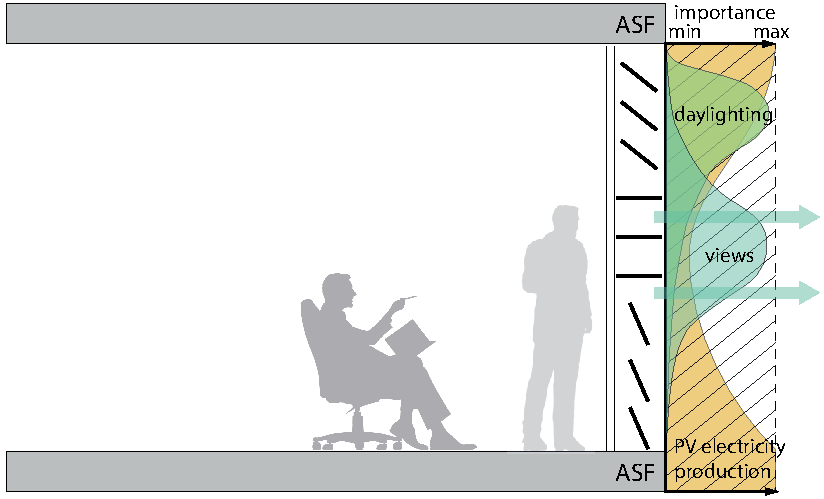
\includegraphics[width=8cm, trim= 0cm 0cm 0cm 0cm,clip]{facadeFunctions.pdf}
\caption{The facade acting as a mediator between the interior and exterior environment, while fullfilling various functions \cite{nagy2015frontiers}}
\label{fig:ASFschematic}
\end{center}
\end{figure}

\begin{figure}
\begin{center}
\includegraphics[width=8cm, trim= 0cm 0cm 0cm 0cm,clip]{honr.jpg}
\caption{An example of an ASF constructed at the House of Natural Resources \cite{nagy2015frontiers}}
\label{fig:HoNR}
\end{center}
\end{figure}

The design of an ASF comes at an added cost. The additional electronics, actuators, and supporting structure adds further embodied CO$_2$ to the product. It is therefore important to conduct a life cycle impact assessment (LCA) to analyse whether the life cycle environmental impacts are favorable, compared to a more classic system. It is also important to see how variations in design can alter the green house gas (GHG) reduction potential of the technology. Aspects such as the chosen actuator, control system, and location of operation can have an impact on environmental performance. 

The state of the art literature assesses existing photovoltaic technologies \cite{raugei2007life} \cite{de2013energy} \cite{fthenakis2011photovoltaics}, and the balance of systems (BOS) which includes all other components of a photovoltaic system \cite{mason2006energy}. This has not however, been expanded to dynamic BIPV systems, and in particular, systems that combine the benefits of adaptive shading and electricity production.\\

%This work has also been expanded to roof mounted BIPV systems \cite{lu2010environmental}. However there is still 

%however this has not yet been expanded to dynamic BIPV systems. \\

In this paper, we investigate the environmental performance of an ASF and compare it to existing static photovoltaic systems. We also investigate 1) a system expansion including the heating ventilation and air conditioning (HVAC) savings through adaptive shading 2) design variations of the ASF, 3) the operational emissions of a building, with and without an ASF, and 4) the sensitivity of the LCA to its location and design.


%In this paper we investigate the trade-off between added material and on-site energy production, along with other benefits such as adaptive shading. We assess 1) the ASF system with possible design variations, 2) the operation of a building with an ASF, 3) its global and local environmental impact, 4) the sensitivity of the LCA to the design and location, and 5) provide a comparison with existing static PV technologies. \\

The remainder of the paper is organized as follows. The following section introduces the ASF and the used LCA methodology. In Section \ref{ch:results}, we present the results of the LCA analysis. Section \ref{ch:discussion} discusses the results and provides design guidelines. Section \ref{ch:conclusion} concludes the paper.


% - In the last decades, building integrated photovoltaics (BIPV) have been adopted as part of the energy strategy towards 2050... \

% (advantages of BIPV, potential of BIPV)\\


% - The current developments of light-weight efficient thin film technologies have brought new design possibilities for architects in BIPV design... \

% (Adaptive Building Envelopes, examples, Envelope is the barrier between the internal and external environment, Advantages, seamless coupling with solar tracking mechanics) \\

% - One example of a multi functional facade that was recently released is the Adaptive Solar Facade.\\

% - The aim of this paper is to analyse the life cycle emissions of an adaptive solar facade and provide comparisons with standard shading systems and static BIPV solutions.\\
